
\documentclass[11pt,titlepage]{article} 
\usepackage[square,sort&compress]{natbib}
%\usepackage[round]{natbib} 
\usepackage{amsfonts}
\usepackage{amsmath}
\usepackage{amssymb}
\usepackage{hyperref}
\usepackage{longtable}


\usepackage{caption}
\captionsetup{labelsep = none}
\usepackage{graphicx,rotating}

\usepackage{setspace}
\usepackage[table]{xcolor}
%\bibliographystyle{elsart-harv}

%\bibliographystyle{JRSS}
\bibliographystyle{genres}
%\usepackage[margin=1in]{geometry}
\newcommand{\mb}[1]{\mathbf{#1}}
\newcommand{\wt}[1]{\widetilde{#1}}
\usepackage{pdfpages}
\doublespacing
\renewcommand{\rmdefault}{ptm} 
\usepackage{mathptmx} 
\usepackage{tikz}
\usetikzlibrary{arrows}
\usepackage[margin=1in]{geometry}
\renewcommand{\baselinestretch}{1.05}    %or 1.4 maybe?
%\setlength{\oddsidemargin}{0cm} \setlength{\textwidth}{6.5in}
%\setlength{\topmargin}{0in} \setlength{\topmargin}{-.5in}
\makeatletter
\renewcommand{\thefigure}{S\@arabic\c@figure}
\makeatother
\makeatletter
\renewcommand{\thetable}{S\@arabic\c@table}
\makeatother

\newcommand\encircle[1]{%
  \tikz[baseline=(X.base)] 
    \node (X) [draw, shape=circle, inner sep=0] {\strut #1};}
%this version seems to work better for pdf (?)
\setlength{\textheight}{9.5in}
%%
%% Select one of the two - the second gets rid of comments.
%% Leave the blank lines in
\def\comment#1{

\smallskip\noindent{\it [{#1}]}

\smallskip\noindent
}
%\def\comment#1{}


\begin{document}
\title{Supplementary Information for: Detection and interpretation of shared genetic influences on 40 human traits}
\author{Joseph K. Pickrell$^{1,2, \dagger}$, Tomaz Berisa${^1}$, Laure Segurel$^{3}$, Joyce Y. Tung${^4}$, David Hinds${^4}$\\ \\
\small $^1$ New York Genome Center, New York, NY, USA\\
\small $^2$ Department of Biological Sciences, Columbia University, New York, NY, USA \\
\small $^3$ CNRS, Paris, France \\
\small $^4$ 23andMe, Inc., Mountain View, CA, USA\\
\small $^\dagger$ Correspondence to: \url{jkpickrell@nygenome.org}
}
\maketitle

\tableofcontents
\clearpage

\section{GWAS data}
In this section, we describe the sources of the GWAS data used in the paper. Overall, for each study, we imputed summary statistics or genotypes for all autosomal variants in the March 2012 release of the 1000 Genomes Phase 1 \citep{abecasis2010map}. Our method uses the Z-scores and standard errors of the estimated effect sizes for each SNP. In studies where standard errors were not provided, we approximated them using the allele frequencies from the European-descent individuals in the 1000 Genomes Phase 1 release and the reported sample size of the study (see \citet{pickrell2013joint} for details). Throughout the paper, we report effect sizes of variants as the effect of the non-reference allele in human genome reference hg19. 
  
\subsection{Previously described in \citet{pickrell2013joint}}
For some phenotypes, the data sources and processing were previously described in \citet{pickrell2013joint}. These are (using the abbreviations from the main text): FG, LDL, HDL, TG, TC,  FNBMD, LSBMD, PLT, MPV, HB, MCHC, RBC, MCV, and PCV. \subsection{Body mass index}
The GIANT consortium GWAS data described in \citet{Locke:2015aa} was downloaded from \url{http://www.broadinstitute.org/collaboration/giant/index.php/GIANT_consortium_data_files}. We removed all SNPs typed on less than 200,000 individuals or more than 240,000 individuals, then performed imputation at the level of the summary statistics. After removing poorly-imputed SNPs (at an $r^2$ threshold less than 0.8), we were left with 6,133,872 summary statistics. To approximate the variance in the effect size estimates, we used a sample size of 240,000 and the allele frequencies estimated from the European-descent individuals in the 1000 Genomes Project. 
\subsection{Waist-hip ratio}
We downloaded summary statistics from the GIANT consortium GWAS of waist-hip ratio corrected for BMI  \citep{Shungin:2015aa} from \url{http://www.broadinstitute.org/collaboration/giant/index.php/GIANT_consortium_data_files}. We used the summary statistics generated using both males and females together. We removed all SNPs genotyped on less than 130,000 individuals or more than 150,000 individuals, then performed imputation at the level of summary statistics.  After removing poorly-imputed SNPs (at an $r^2$ threshold less than 0.8), we were left with 5,859,436 summary statistics. To approximate the variance in the effect size estimates, we used a sample size of 142,762 and the allele frequencies estimated from the European-descent individuals in the 1000 Genomes Project. 

\subsection{Coronary artery disease}
The CARDIoGRAM GWAS data described in \citet{Schunkert:2011aa} was downloaded from \url{http://www.cardiogramplusc4d.org/downloads/}. We removed all SNPs typed on less than  15,000 cases or 50,000 controls, then imputed summary statistics for all SNPs in the 1000 Genomes Phase 1 release using ImpG \citep{pasaniuc2013fast}. After removing poorly-imputed SNPs (at an $r^2$ threshold less than 0.8), we were left with 5,768,612 summary statistics on an average of around 15,000 cases and 50,000 controls. To approximate the variance in the effect size estimates we used the allele frequencies from the European-descent individuals in the 1000 Genomes Project. 

\subsection{Crohn's disease}
We obtained updated versions of the summary statistics from the GWAS described in \citet{jostins2012host} from \url{http://www.broadinstitute.org/~sripke/share_links/KMaiXtod0Alvozgg5oJgl3QK7VVH2N_IBD_0711a/}, and processed them as described previously \citep{pickrell2013joint}.  After imputation, we had 6,065,937 summary statistics.

\subsection{Type 2 diabetes}
The DIAGRAM consortium summary statistics described in \citep{Morris:2012aa} were downloaded from \url{http://diagram-consortium.org/downloads.html}. We removed SNPs typed on less than 9,000 cases or 50,000 controls, then imputed summary statistics for all variants in the 1000 Genomes Phase 1 release. After imputation, we had 5,824,487 summary statistics. To approximate the variance in the effect size estimates we used the allele frequencies from the European-descent individuals in the 1000 Genomes Project. 

\subsection{Alzheimer's disease}
Summary statistics from the IGAP (International Genomics of Alzheimer?s Project) consortium GWAS \citep{Lambert:2013aa} were downloaded from \url{http://www.pasteur-lille.fr/en/recherche/u744/igap/igap_download.php}. As per the description of the data:

\begin{quote}
International Genomics of Alzheimer's Project (IGAP) is a large two-stage study based upon genome-wide association studies (GWAS) on individuals of European ancestry. In stage 1, IGAP used genotyped and imputed data on 7,055,881 single nucleotide polymorphisms (SNPs) to meta-analyse four previously-published GWAS datasets consisting of 17,008 Alzheimer's disease cases and 37,154 controls (The European Alzheimer's disease Initiative - EADI the Alzheimer Disease Genetics Consortium - ADGC The Cohorts for Heart and Aging Research in Genomic Epidemiology consortium - CHARGE The Genetic and Environmental Risk in AD consortium - GERAD). In stage 2, 11,632 SNPs were genotyped and tested for association in an independent set of 8,572 Alzheimer's disease cases and 11,312 controls. Finally, a meta-analysis was performed combining results from stages 1 \& 2.
\end{quote}

We used only the stage 1 results in all analysis. 

\subsection{Schizophrenia}
Summary statistics from the psychiatric genomics consortium GWAS \citep{Schizophrenia-Working-Group-of-the-Psychiatric-Genomics-Consortium:2014aa} were downloaded from \url{http://www.med.unc.edu/pgc/downloads}. The data consist of summary statistics at 9,444,231 variants.

\subsection{Height}
Summary statistics from the GIANT consortium GWAS \citep{Wood:2014aa} were downloaded from \url{http://www.broadinstitute.org/collaboration/giant/index.php/GIANT_consortium_data_files}. We removed all SNPs with a sample size less than 230,000, then imputed summary statistics for all variants in the 1000 Genome Phase 1 release. After imputation, we had 6,021,095 summary statistics. To approximate the variance in the effect size estimates, we used a sample size of 230,000 and allele frequencies from the European individuals in the 1000 Genomes Project.

\subsection{Age at menarche}
Summary statistics from the Reprogen consortium GWAS \citep{Perry:2014aa} were downloaded from \url{http://www.reprogen.org/data_download.html}. We imputed summary statistics for all variants in the 1000 Genome Phase 1 release. After removing poorly-imputed SNPs, we had 6,277,050 summary statistics. To approximate the variance in the effect size estimates, we used a sample size of 132,989 and the allele frequencies from the European-descent individuals in the 1000 Genomes Project. 


\subsection{Rheumatoid arthritis}
Summary statistics from \url{http://plaza.umin.ac.jp/~yokada/datasource/files/GWASMetaResults/}. We used the GWAS conducted in European-descent individuals only. These data consist of 8,747,963 summary statistics.

\subsection{23andMe data} 
GWAS for a number of traits were performed by the personal genomics company 23andMe using a survey design \citep{Eriksson:2010aa}. Some of these GWAS have been partially described previously \citep{Eriksson:2012ab, Eriksson:2012aa, Eriksson:2010aa, Do:2011aa, Kiefer:2013aa}. Details of each GWAS are described in separate Supplementary Notes.

We used filters and summary data described in these Supplementary Notes, with two exceptions: for both allergies and Parkinson's disease, we used more stringent thresholds for genotyping batch effects. Specifically, 23andMe reports a P-value for whether the allele frequencies of each SNP are associated to genotyping batch or to imputation batch. We used P-value thresholds of $P = 1\times 10^{-7}$ and $1\times10^{-6}$, respectively, for these two studies. This more stringent cutoff was used to account for an imbalance in the enrollment of cases versus controls over time in these two studies. Some small residual batch effect likely explains the small correlation in effect sizes between Parkinson's disease and allergies in Figure 4 in the main text.

%\subsubsection{Age at menarche}
%\includepdf[pages=1-5]{23andMe_phenos/AAM.pdf}

%\subsubsection{Age at voice drop}
%\includepdf[pages=1-4]{23andMe_phenos/AVD.pdf}

%\subsubsection{Allergies}
%\includepdf[pages=-]{23andMe_phenos/ALL.pdf}
%\subsubsection{Asthma}
%\includepdf[pages=-]{23andMe_phenos/ATH.pdf}
%\subsubsection{Beighton hypermobility}
%\includepdf[pages=-]{23andMe_phenos/BHM.pdf}

%\subsubsection{Childhood ear infections}
%\includepdf[pages=-]{23andMe_phenos/CEI.pdf}

%\subsubsection{Breast size}
%\includepdf[pages=-]{23andMe_phenos/CUP.pdf}
%\subsubsection{Chin dimples}
%\includepdf[pages=-]{23andMe_phenos/DIMP.pdf}
%\subsubsection{Hypothyroidism}
%\includepdf[pages=-]{23andMe_phenos/HTHY.pdf}

%\subsubsection{Migraine}
%\includepdf[pages=-]{23andMe_phenos/MIGR.pdf}

%\subsubsection{Male pattern baldness}
%\includepdf[pages=-]{23andMe_phenos/MPB.pdf}

%\subsubsection{Nose size}
%\includepdf[pages=-]{23andMe_phenos/NOSE.pdf}

%\subsubsection{Nearsightedness}
%\includepdf[pages=-]{23andMe_phenos/NST.pdf}

%\subsubsection{Parkinson's disease}
%\includepdf[pages=-]{23andMe_phenos/PD.pdf}

%\subsubsection{Photic sneeze reflex}
%\includepdf[pages=-]{23andMe_phenos/PS.pdf}

%\subsubsection{Tonsillectomy}
%\includepdf[pages=-]{23andMe_phenos/TS.pdf}

%\subsubsection{Unibrow}
%\includepdf[pages=-]{23andMe_phenos/UB.pdf}


\section{Additional details about the hierarchical model}
We ran the hierarchical model as described in the main text on all pairs of phenotypes. In this section we describe simulations and additional complications that we did not account for in the main analyses.

\subsection{Comparison to Stephens's Bayes factors}

There are a number of existing approaches to testing for an association between a genetic variants and multiple traits \citep{Zhang:2014aa, Stephens:2013fk, OReilly:2012aa, Ferreira:2009aa, Zhou:2014aa, Korte:2012aa}. The most similar approach to ours is that of \citet{Stephens:2013fk}. We compared the qualitative performance of the two (SNP-level) Bayes factors using simulations. Recall that there are three possible non-null models for each SNP: either it influences 1) the first trait alone, 2) the second trait alone, or 3) both traits. The simulation algorithm was as follows:

\begin{enumerate}
\item Simulate an effect size: $\beta \sim N(0, 0.09)$ and an allele frequency $f \sim Beta(2,2)$.
\item Simulate 5,000 genotypes: $\vec g = [g_1, g_2, ... g_{5000}]$, where \\ $g_i \sim Bin(2, f)$.
\item Simulate a pair of phenotypes for each simulated genotype according to one of the models described above: $[x_i, y_i] \sim MVN(\vec \mu, \Sigma)$, where $\mu_1 = g_i \beta$ if simulating from models 1 or 3 (and zero otherwise), $\mu_2 = g_i \beta$ if simulating from models 2 or 3 (and zero otherwise) and $\Sigma$ is a variance/covariance matrix with the diagonal set to one and the off-diagonal terms set to a correlation $C$.
\item Calculate the Bayes factors measuring the evidence in favor of each of the three alternative models using their the Bayes factors as described in the main text or the code in Supplementary Section 3 of \citet{Stephens:2013fk}. We used a prior variance of 0.5, and estimated the correlation in the phenotypes directly from the simulated phenotypes (rather than setting it to the simulated value).
\end{enumerate}

\paragraph{Results.} We considered two correlation coefficients (0 and -0.4) and all three possible alternative models, for a total of six simulation conditions. In each condition, we repeated the procedure above 1,000 times and calculated all three possible Bayes factors. For example, in the condition where the ``truth" is two uncorrelated phenotypes and a genetic variant that influences only the first, we calculated Bayes factors measuring the support for the true model (model 1: only the first phenotype is associated with the genotype) as well as the Bayes factor supporting the model 2 (only the second phenotype is associated with the genotype) and the Bayes factor measuring the support for model 3 (both phenotypes are associated with the genotype). 

In Figure \ref{f_c0}, we show our Bayes factors and the Stephens Bayes factors for the situation where the two phenotypes are uncorrelated. The two Bayes factors are similar in all situations. In Figure \ref{f_c-4}, we show our Bayes factors and the Stephens Bayes factors for the situation where the two phenotypes are (negatively) correlated. The two Bayes factors disagree considerably in two situations. Specifically, in simulations where a genetic variant is associated with only a single phenotype and the test is for association with the \emph{other} phenotype, our Bayes factors show little-to-no evidence for association, while the Stephens Bayes factors sometimes show substantial evidence for association. On reflection, this appears to be due to a small but apparently important difference in underlying models. Specifically, the \citet{Stephens:2013fk} model is equivalent for testing for independence between the genotype and the second phenotype \emph{conditional} on the first phenotype, while we are testing for \emph{unconditional} independence between the genotype and the phenotype.  

 
\begin{figure}
\begin{center}
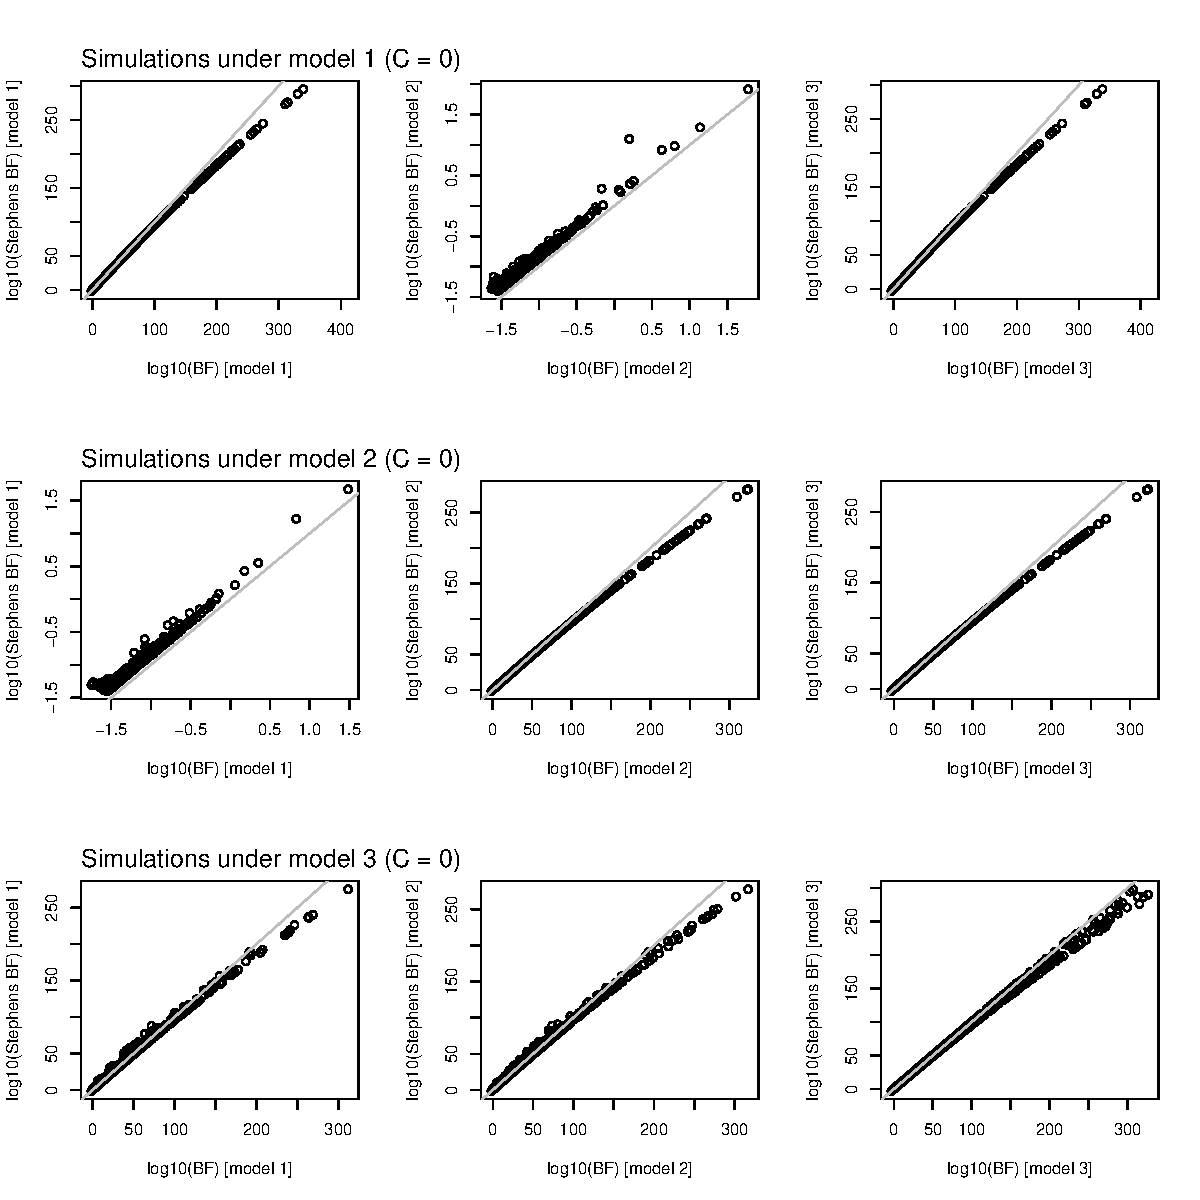
\includegraphics[scale = 0.6]{figs/allc0.pdf}
\caption{. \textbf{Comparison to Stephens' Bayes factor for uncorrelated traits.} We simulated genotypes and phenotypes for 5,000 individuals, and compared the approximate Bayes factor used here to that from \citet{Stephens:2013fk}. In each panel, each point is a single simulation. }\label{f_c0}
\end{center}
\end{figure}

\begin{figure}
\begin{center}
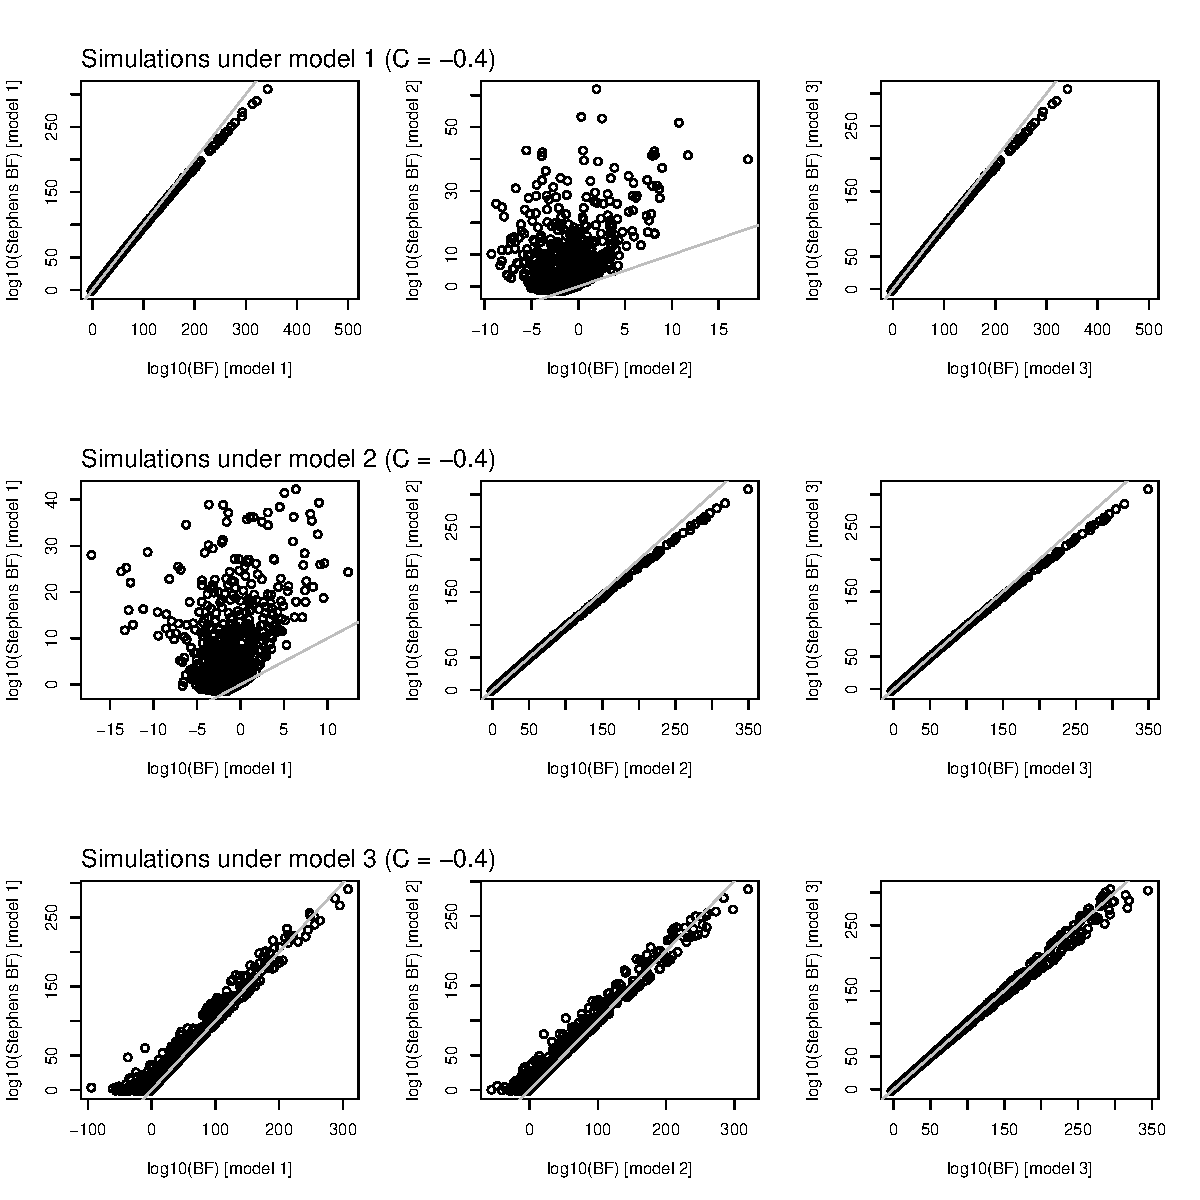
\includegraphics[scale = 0.6]{figs/allc-4.pdf}
\caption{. \textbf{Comparison to Stephens' Bayes factor for correlated traits.} We simulated genotypes and phenotypes for 5,000 individuals, and compared the approximate Bayes factor used here to that from \citet{Stephens:2013fk}. In each panel, each point is a single simulation.}\label{f_c-4}
\end{center}
\end{figure}



\subsection{Simulations}
We wanted to evaluate the performance of the hierarchical model in moderately realistic simulations. To do this, we simulated GWAS using haplotypes from the HapMap Project \citep{Frazer:2007dz}. We predefined 111 genomic regions to simulate data from, and assigned two genetic variants in each region as the potentially causal variants (see Figure 1 in the main text). Each simulation then had the following steps:

\begin{enumerate}
\item Simulate 10,000 haplotypes in the 111 genomic regions using hapgen2 \citep{Su:2011aa} and reference haplotypes from the HapMap Project. 
\item Assign each region to one of the five models $RM_{[0-4]}$ randomly (in general, we evenly distributed the regions to all five models).
\item Sum the number of causal alleles for both phenotypes for each individual (combining two simulated haplotypes to make an individual).
\item Simulate phenotypes for each individual as $MVN(\mu, \Sigma)$ (where $\mu$ and $\Sigma$ were set as described below) and quantile normalize the phenotypes. 
\item Run linear regression of each SNP against both phenotypes (in simulations of separate cohorts, we used half the individuals for the association study of the first phenotype, and half for the association study of the second).
\item Run the model on the summary statistics generated from these linear regressions. For all runs, we used a prior variance on the effects sizes of 0.5.
\end{enumerate}

\subsubsection{Simulated traits}
For uncorrelated traits, we simulated the phenotypes of each individual as independent normally distributed variables with $\mu = 0.3 n_i$, where $n_i$ is the counts of causal alleles for phenotype $i$, and $\sigma^2 = 0.1$. For simulations of correlated traits, we used the same structure, except that we set the covariance between the two phenotypes as $0.1*\rho$, where $\rho$ was set according to the simulation.

\begin{figure}
\begin{center}
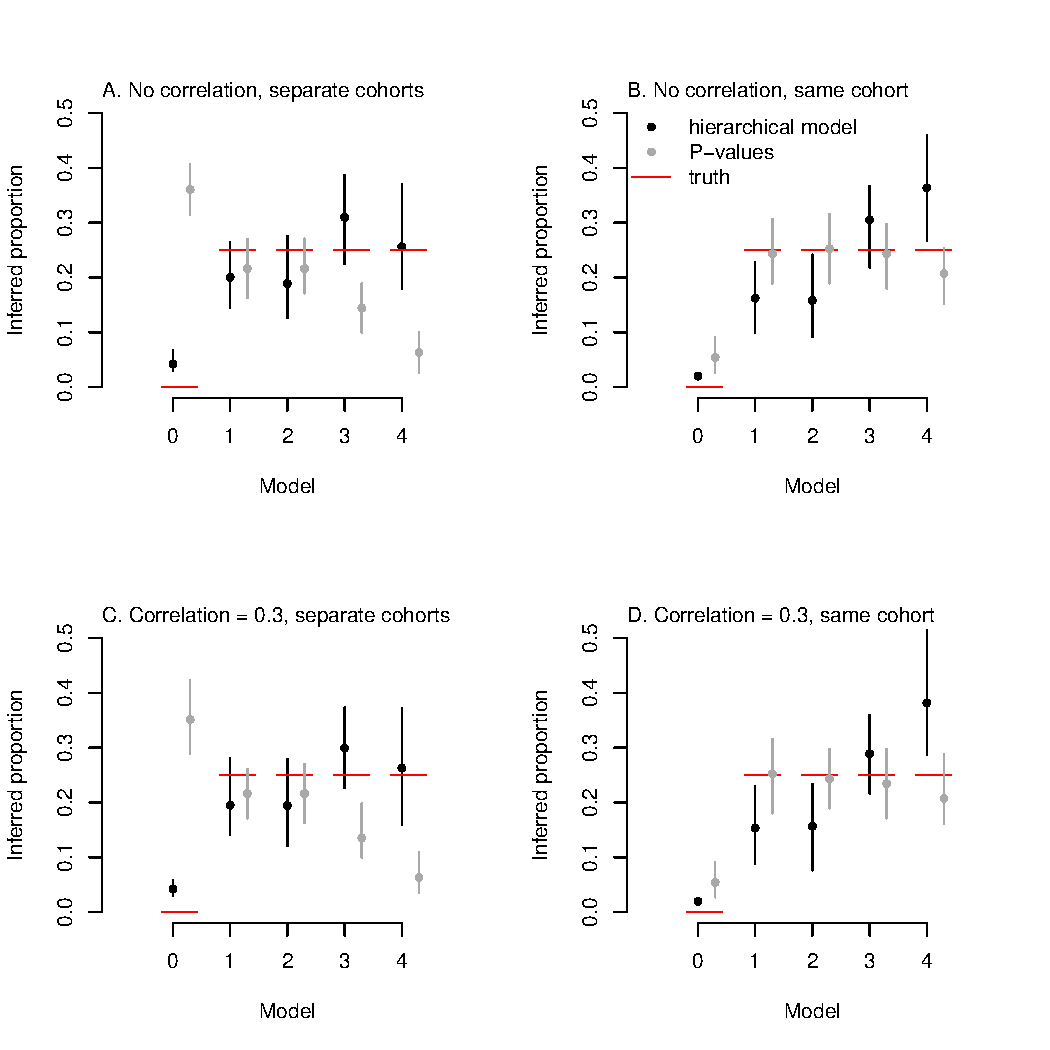
\includegraphics[scale = 0.6]{figs/sims.pdf}
\caption{. \textbf{Simulations.} We simulated GWAS under four different assumptions, and then compared our model to a simple P-value based model. In each panel, we show the simulated values of $\Pi_{[0-4]}$ and the estimated values. Each point is the mean over 100 simulations, and the bars show the 5-95\% range of parameter values obtained over these 100 simulations. \textbf{A.} Simulations of uncorrelated phenotypes in separate cohorts. \textbf{B.} Simulations of uncorrelated phenotypes in overlapping cohorts. \textbf{C.} Simulations of correlated phenotypes in separate cohorts. \textbf{D.} Simulations of correlated phenotypes in overlapping cohorts.}\label{f_sim}
\end{center}
\end{figure}

\begin{figure}
\begin{center}
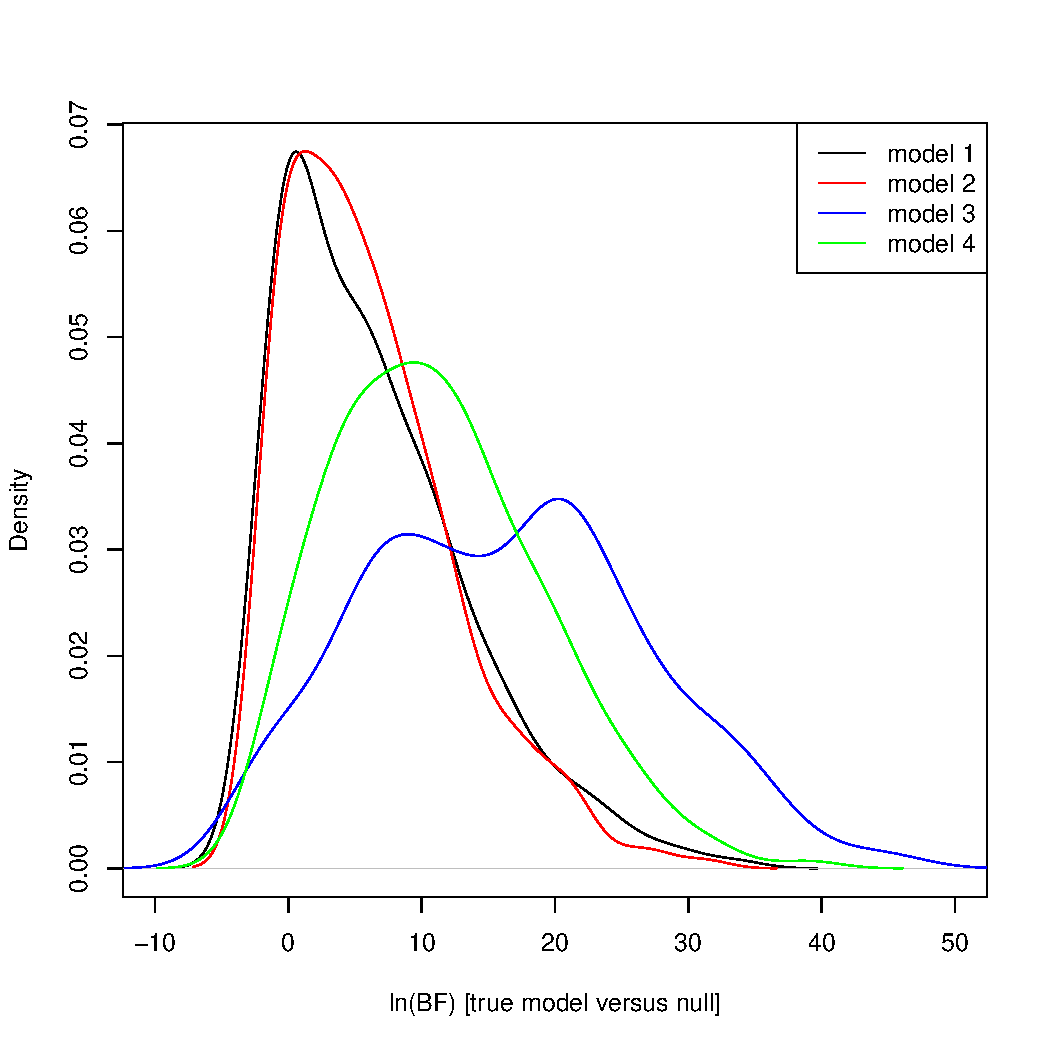
\includegraphics[scale = 0.6]{figs/bfs_sim.pdf}
\caption{. \textbf{Regional Bayes factors in simulations.} For ten simulations (recall that each simulation consists of 111 regions) of separate cohorts and uncorrelated traits, we extracted all regional Bayes factors, and grouped regions according to the model under which each was simulated. We then plot the distribution of the regional Bayes factors under the ``true" model. That is, for regions simulated under regional model 1, we show the distribution of $RBF_1$, for regions simulated under regional model 2, we show the distribution of $RBF_2$, and so on. Note that the distribution is shifted to the right for regions simulated under model 3 (a single genetic variant that influences both traits), indicating that there is more evidence against the null model of no associations in this situation.}\label{f_bfsim}
\end{center}
\end{figure}


\subsubsection{Results}
We simulated four situations: uncorrelated traits (both overlapping cohorts and non-overlapping cohorts) and correlated traits (both overlapping cohorts and non-overlapping cohorts) with a correlation coefficient of 0.3. Shown in Supplementary Figure \ref{f_sim} are the parameter estimates obtained in the simulations. For comparison, we also used a simple P-value model where a region was called a ``hit" for each phenotype if a SNP had a P-value of less than $5\times 10^{-8}$ for the phenotype. If a single variant had a P-value less than $5\times10^{-8}$ for one phenotype and a P-value less than $5\times10^{-5}$ for the other phenotype, we called this as fitting model 3 (of co-localized signals). 

We see that in the case of separate cohorts (Supplementary Figure \ref{f_sim}A,C), the hierarchical model gets close to the truly simulated proportions, while the P-value method dramatically overestimates $\Pi_0$. There is a slight overestimation of $\Pi_3$, which we attribute the fact that the evidence against the null for variants that truly influence both phenotypes is stronger than for variants that influence only a single trait. In the case of perfectly overlapping cohorts (Supplementary Figure \ref{f_sim}B,D), the hierarchical model additionally overestimates $\Pi_4$, likely for the reason discussed below. In this case the P-value method performs well, though we attribute this to the fact that we have simulated a GWAS where all variants have the same effect size and the sample size is large enough to have excellent power to detect this effect size. In real GWAS, this is unlikely to be the case.

\subsection{Accounting for linkage disequilibrium in overlapping cohorts}
In the main text, we describe the hierarchical model used in the main analyses that accounts for overlapping cohorts by modeling the correlation in the phenotypes. Here were describe an approach to account for linkage disequilibrium as well. This is only relevant for the calculation of the Bayes factor measuring the support for regional model 4, where there are two causal variants in a region, one of which influences the first phenotype and one of which influences the second phenotype.

\subsubsection{Conditional Bayes factors.} \label{conditional_bfs}
In this situation, it is necessary to approximate a conditional regression analysis--that is, to estimate the effect size of one genetic variant conditional on the estimated effect size of another genetic variant. We redefine some notation for simplicity. Consider a single phenotype and two genetic variants. Let $\vec y$ be a vector of (standard normally-distributed) phenotypes, $\vec g_{1}$ be the mean-centered vector of genotypes at SNP 1, $\vec g_{2}$ be the mean-centered vector of genotypes at SNP 2, $\hat \beta_1$ be the (non-conditional) estimate of the effect of SNP 1 on the phenotype from a simple linear regression of the phenotype on the genotypes at SNP 1, and $\hat \beta_2$ be the analogous estimate for SNP 2. We consider the conditional regression model where:

\begin{equation}
y_i - \hat \beta_2 g_{i2} =  \beta_1^{\prime} g_{i1} + \epsilon,
\end{equation}

\noindent where  $\beta_1^{\prime}$ is the conditional estimate of the effect size of SNP 1 and $i$ indexes individuals. The least squares estimate of this effect size is:

\begin{align}
\hat \beta_1^{\prime} &= \frac{\sum \limits_i (y_i - \hat \beta_2 g_{i2})  g_{i1}}{ \sum \limits_i g_{i1}^2} \\
\hat \beta_1^{\prime} &= \hat \beta_1 - \frac{Cov(g_1, g_2)}{Var(g_1)} \hat \beta_2,
\end{align}
\noindent In order to compute our approximate Bayes factors, we need the variance in this estimate. If we let $R = \frac{Cov(g_1, g_2)}{Var(g_1)}$:

\begin{align}
Var(\hat \beta_1^{\prime}) &= Var( \hat \beta_1 - R \hat \beta_2)\\
&= Var(\hat \beta_1) + Var(R \hat \beta_2) - 2 Cov (\hat \beta_1, R \hat \beta_2) \label{vB}.
\end{align}
If we assume that there is no error in our estimate of $R$, this reduces to:

\begin{align}
Var(\hat \beta_1^{\prime}) \approx Var(\hat \beta_1) - R^2 Var( \hat \beta_2),
\end{align}

\noindent which is equivalent to Equation 20 from \citet{Yang:2012uq} (assuming effect sizes are small, such that the residual variance is equivalent to the phenotypic variance). We can then define $Z^{\prime} = \frac{\hat \beta_1^{\prime}}{\sqrt{ Var(\hat \beta_1^{\prime})}}$ and use any of the approximate Bayes factors as defined previously. 

\paragraph{Propagating error in $R$.} It has been suggested that if $R$ is estimated from around 2,000 individuals then it can be treated as a scalar rather than a random variable \citep{Yang:2012uq}. In general, however, we do not have access to the genotype data underlying a study, so we will estimate $R$ from a separate panel of publicly-available haplotypes from individuals of the same ancestry as the individuals in the association study. These panels generally have hundreds rather than thousands of individuals, so we need to propagate the error in $R$. Under the null, the second term in Equation \ref{vB} is:

\begin{equation}
Var(R \hat \beta_2) = E[R]^2 Var( \hat \beta_2) + 2 Var(\hat \beta_2) Var(R),
\end{equation}

\noindent and the third is:
\begin{align}
Cov (\hat \beta_1, R \hat \beta_2) &= E[ R  \hat \beta_1 \hat \beta_2]\\
& = R Cov (\hat \beta_1, \hat \beta_2)\\
& = R^2 Var(\hat \beta_2),
\end{align}

\noindent so substituting and simplifying we get:

\begin{equation} \label{varB}
Var(\hat \beta_1^{\prime}) = Var(\hat \beta_1) + Var(\hat \beta_2) [2 Var(R)- R^2].
\end{equation}

Finally, we need to approximate the variance in $R$. We assume this is estimated from a reference panel consisting of $2M$ phased haplotypes from $M$ diploid individuals. Let the count of haplotypes carrying the non-reference alleles at both sites be $c_{11}$, the count of haplotypes carrying the reference allele at the first site and the non-reference allele at the second site be $c_{10}$, and so on for $c_{01}$ and $c_{00}$. We define the analogous frequencies $f_{11}, f_{10}, f_{01}$, and $f_{00}$. With this notation, $\hat R = \frac{f_{11} - (f_{10}+f_{11})(f_{01}+f_{11})}{ (f_{10}+f_{11})(1-(f_{10}+f_{11}))}$.   Using the delta method \citep{Agresti:2002vk}:  

\begin{equation}
Var (\hat R) \approx \Delta \Sigma \Delta^{T},
\end{equation} 
\noindent where $\Delta$ is the vector of partial derivatives of $\hat R$ with respect to $f_{11}, f_{10}$, and  $f_{01}$, and $\Sigma$ is the covariance matrix of these frequencies. Explicitly, $\Delta$ is:

\begin{align}
\frac{\partial \hat R}{\partial f_{11}} &= \frac{f_{10} (1-f_{1.})^2 - f_{01} f_{1.}^2}{f_{1.}^2 (1-f_{1.})^2}  \\
 \frac{\partial \hat R}{\partial f_{10}} &= \frac{-f_{01}f_{1.}^2 - f_{11} (1-f_{1.})^2}{f_{1.}^2 (1-f_{1.})^2}\\
 \frac{\partial \hat R}{\partial f_{01}} &= \frac{1}{f_{1.}-1}, 
\end{align}
\noindent where $f_{1.} = f_{11}+f_{10}$. Additionally, $\Sigma$ is:

\begin{equation}
Cov(f_i, f_j) =
  \begin{cases}
   \frac{f_i (1-f_i)}{2M} & \text{if } i = j \\
   \frac{- f_i f_j}{2M}       & \text{if } i \ne j
  \end{cases}.
\end{equation}
We can thus calculate $Var(\hat R)$, and plug this into Equation \ref{varB} to estimate the variance in the estimate of the conditional effect size. 
\paragraph{Multivariate conditional Bayes factors.} We note that the above calculation are for a single phenotype. For two phenotypes, we simply perform the above procedure for each individually. This gives a corrected Z-score for each of the two phenotypes, which can then be plugged into any of the calculations for our approximate Bayes factors. 

\subsubsection{Regional Bayes factors}
We can now write down the Bayes factors measuring the support for an association in a given genomic region $r$. As in the situation where the two traits have been measured in separate cohorts,

\begin{align}
RBF_r^{(1)} &= \sum \limits_{i = 1}^{K} \pi_i^{(1)} BF_i^{(1)}\\
RBF_r^{(2)}  &= \sum \limits_{i = 1}^{K} \pi_i^{(2)} BF_i^{(2)} \\
RBF_r^{(3)}  &= \sum \limits_{i = 1}^{K} \pi_i^{(3)} BF_i^{(3)} \\
RBF_r^{(4)}  &= \sum \limits_{i = 1}^{K} \sum \limits_{j = 1}^K \pi_i^{(1)} \pi_j^{(2)}  BF_i^{(1)} BF_j^{\prime(2)} I[i \ne j ],\\
\end{align} 

\noindent where $I[i \ne j]$ is an indicator that evaluates to 1 if $i$ and $j$ are different and 0 otherwise,  $\pi_i^{(1)}$ is the prior probability that SNP $i$ is the causal SNP under model 1, $\pi_i^{(2)}$ is the prior probability that SNP $i$ is the causal SNP under model 2, and $\pi_i^{(3)}$ is the prior probability that SNP $i$ is the causal SNP under model 3. Additionally, $BF_j^{\prime(2)}$ is the Bayes factor at SNP $j$ conditional on the observed effects at SNP $i$, calculated using the procedure in Section \ref{conditional_bfs}. Note the only difference to the method in the main text is the calculation of $RBF_r^{(4)}$.

\subsubsection{Application}
We applied this method to several genome-wide association studies that we know were performed on the same cohorts. We calculated $R_{ij}$ between all pairs of SNPs using the haplotypes from the European-descent individuals in the 1000 Genomes Project as $\frac{\hat V_{ij}}{\hat V_{ii}}$, where both of these were estimated using the shrinkage estimator of \citet{Wen:2010aa} and the recombination rate estimates from the HapMap Project. We ran the model in three modes: 1) assuming the cohorts were completely separate, 2) accounting for the correlation in the summary statistics under the null but not linkage disequilibrium, and 3) accounting for both the correlation in the phenotypes and linkage disequilibrium. Shown in Supplementary Figure \ref{f_barplot} are the parameter estimates in these three situations for four pairs of GWAS. In general, correcting for LD made little difference in practice. For all of the main analyses, we only corrected for the correlation in summary statistics under the null.


\begin{figure}
\begin{center}
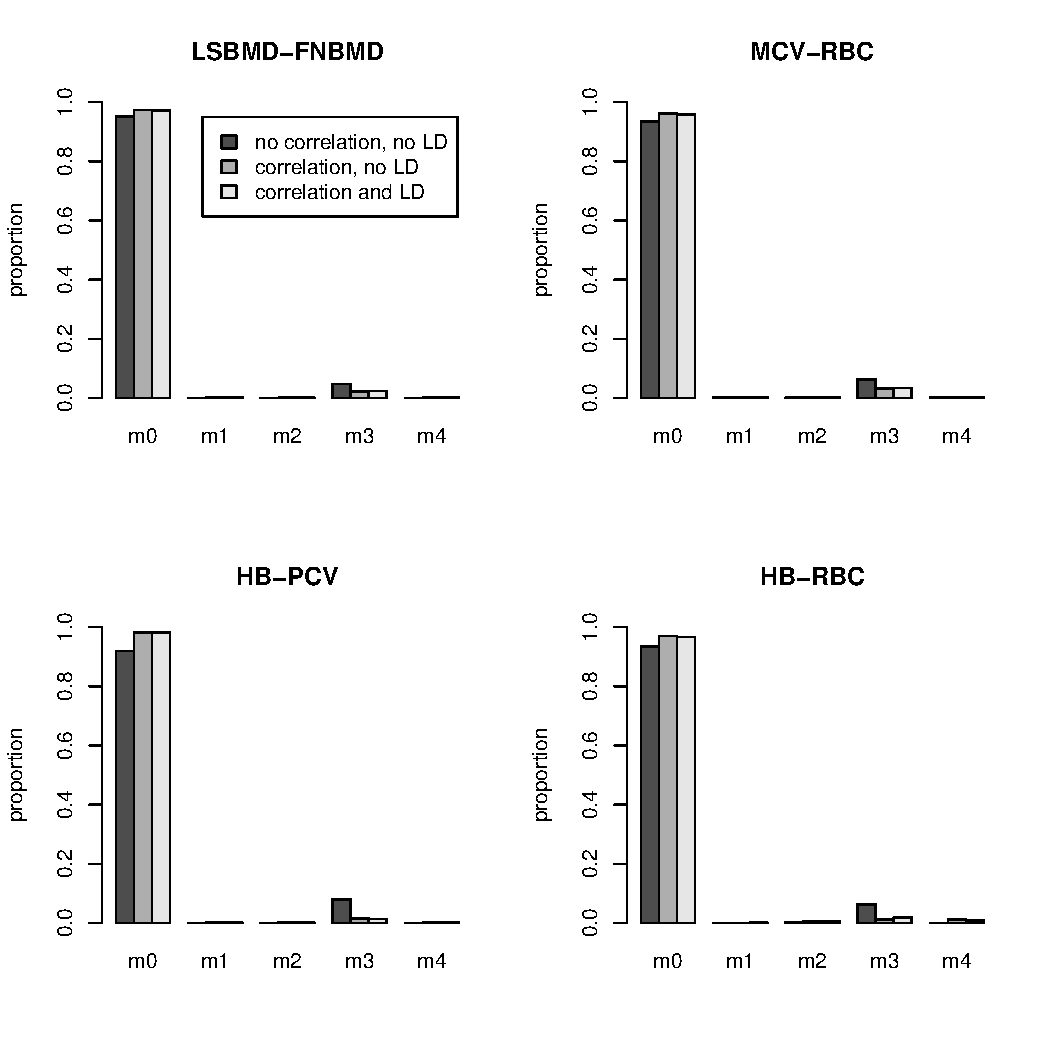
\includegraphics[scale = 0.6]{figs/barplot.pdf}
\caption{. \textbf{Parameter estimates in select GWAS accounting for different factors.} For the noted pairs of GWAS (which we know to have been performed on overlapping sets of individuals), we ran the model in modes where we either 1) corrected for neither the correlation in the summary statistics under the null nor for LD, 2) corrected for the correlation in the summary statistics alone, or 3) corrected for both the correlation in the summary statistics and LD. Shown are the parameter estimates for these three situations.}\label{f_barplot}
\end{center}
\end{figure}

\begin{figure}
\begin{center}
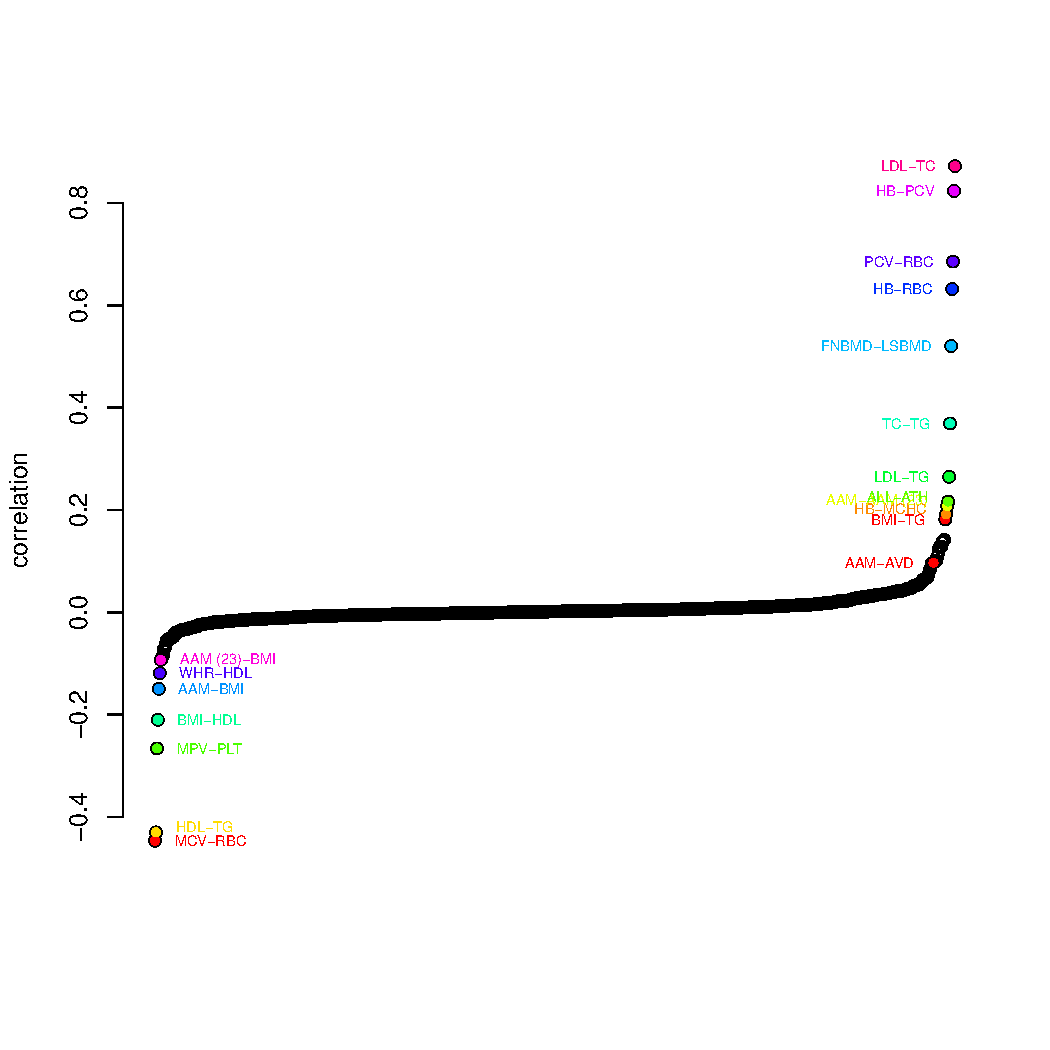
\includegraphics[scale = 0.6]{figs/cor.pdf}
\caption{. \textbf{Correlations in Z-scores.} For each pair of GWAS, we identified regions with low posterior probability of having a causal variant for either trait, and then calculated the correlation in the Z-scores for SNPs in these regions. Shown are the estimated correlations for all pairs of traits, ordered from lowest to highest. Some pairs of note are in color.}\label{f_cor}
\end{center}
\end{figure}

\begin{figure}
\begin{center}
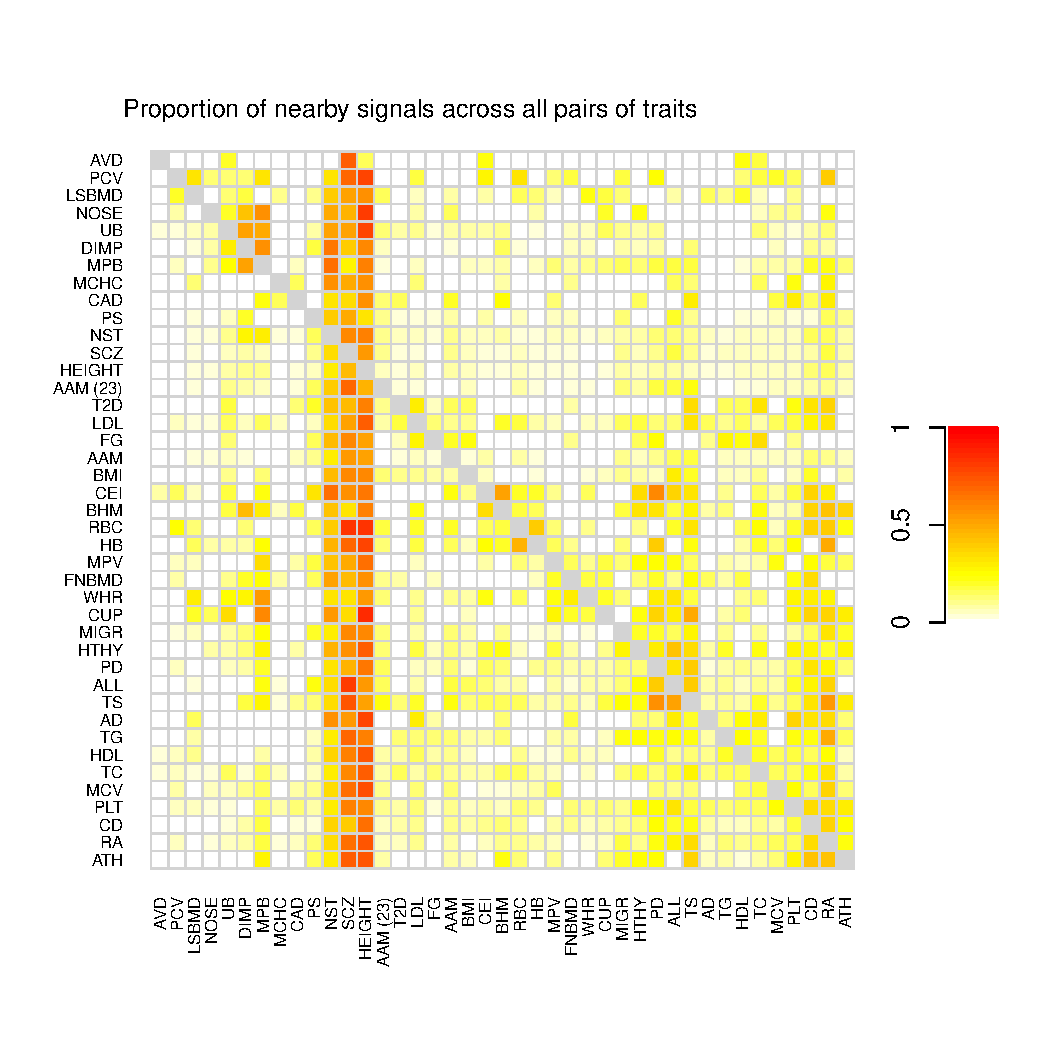
\includegraphics[scale = 0.6]{figs/heatmap_pi4.pdf}
\caption{. \textbf{Heatmap showing how often loci that influence two traits fall near each other in the genome.} Each square $[i,j]$ shows the maximum \emph{a posteriori} estimate of the proportion of genetic variants that influence trait $i$ that fall near a variant that influence trait $j$ (in the notation from the main text, this is $\frac{\hat \Pi_4}{\hat \Pi_1 + \hat \Pi_3 + \hat \Pi_4}$). Note that this is not symmetric. Darker colors represent larger proportions. Colors are shown for all pairs of traits that have at least one region with a posterior probability of model 4 greater than 0.9.}\label{f_pi4}
\end{center}
\end{figure}

\begin{figure}
\begin{center}
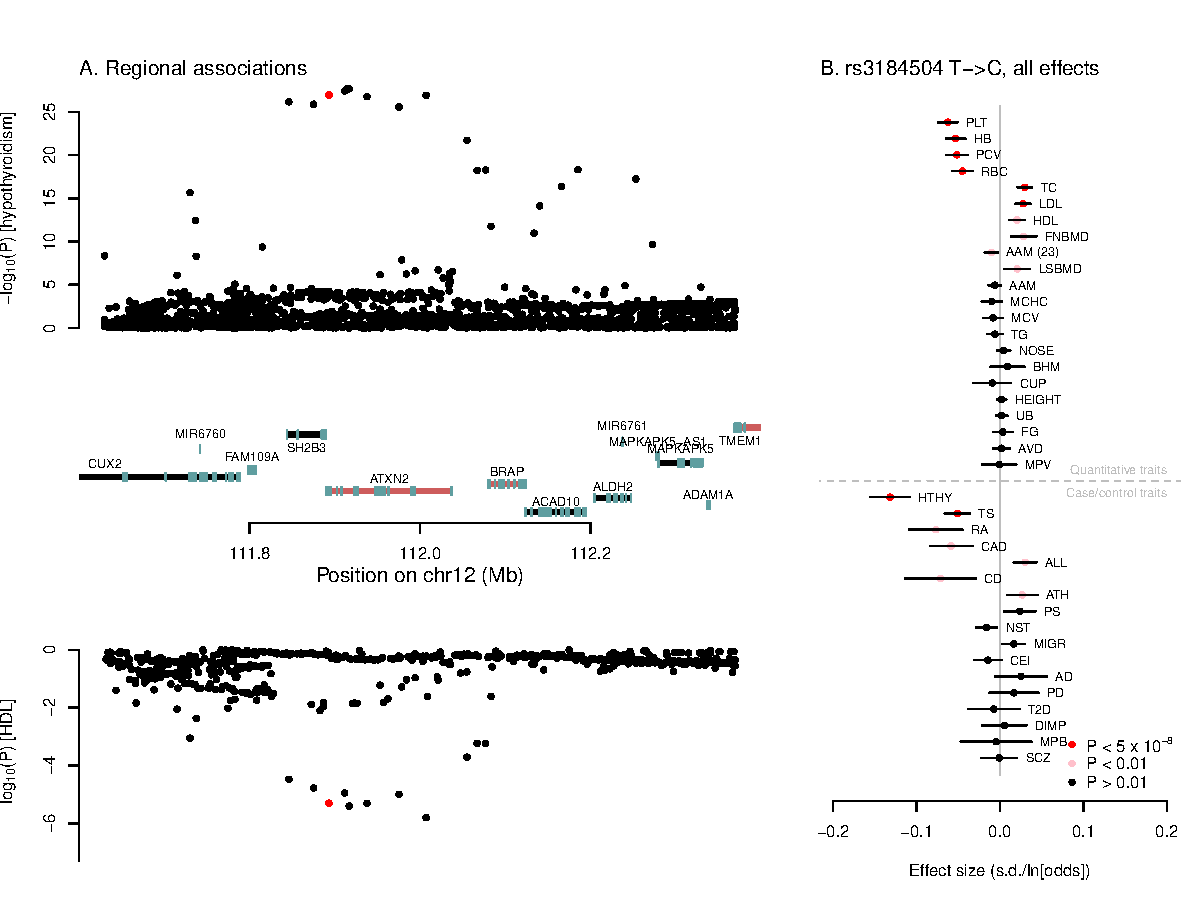
\includegraphics[scale = 0.6]{figs/SH2B3_region.pdf}
\caption{. \textbf{SH2B3 region. A. Regional association signals.} Shown are the P-values for association in the region for hypothyroidism and HDL cholesterol levels. In red is the nonsynonymous SNP rs3184504. \textbf{B. Effect of rs3184504 on all phenotypes.} Shown are the effects of the C allele on all phenotypes where this variant was successfully genotypes or imputed. Bars represent 95\% confidence intervals. }\label{f_sh2b3}
\end{center}
\end{figure}

\begin{figure}
\begin{center}
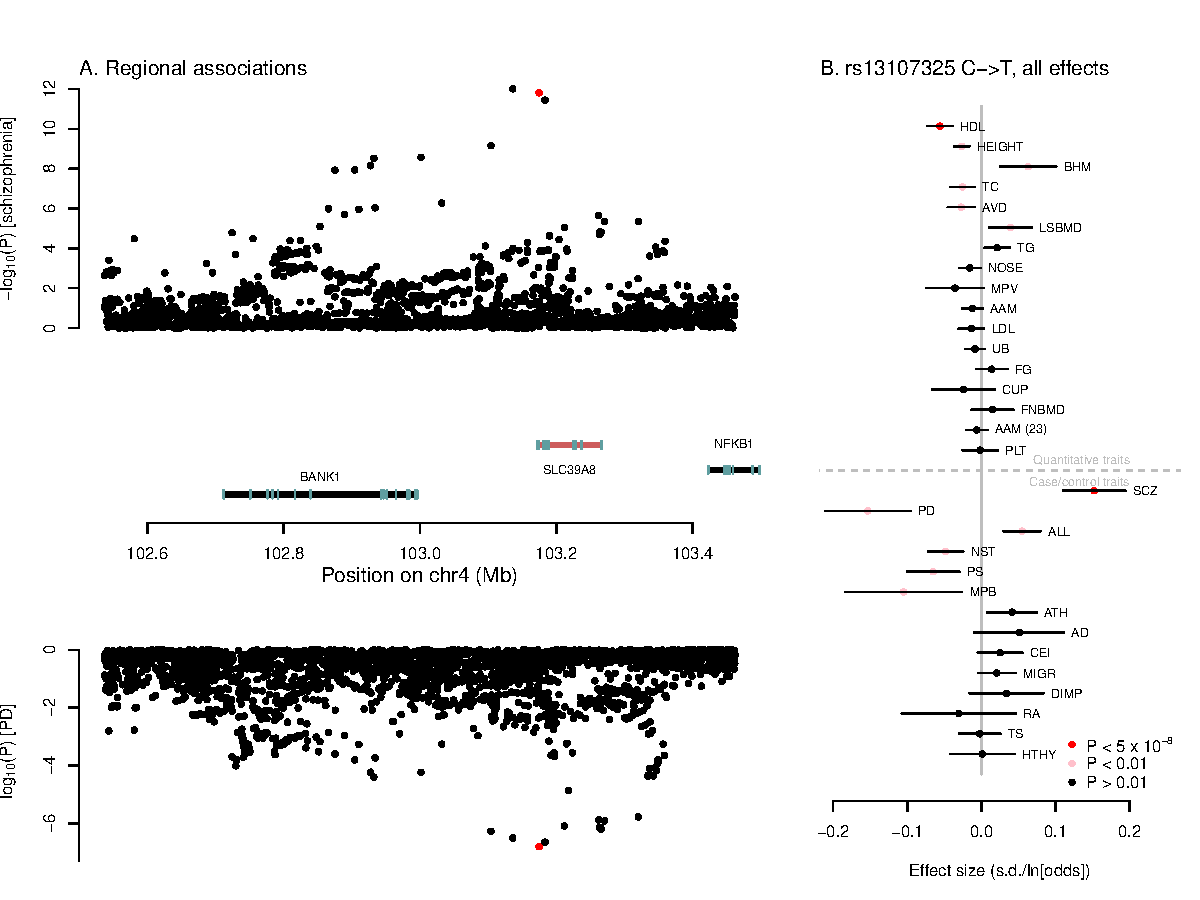
\includegraphics[scale = 0.6]{figs/SLC39A8_region.pdf}
\caption{. \textbf{SLC39A8 region. A. Regional association signals.} Shown are the P-values for association in the region for schizophrenia and Parkinson's disease. In red is the nonsynonymous SNP rs13107325. \textbf{B. Effect of rs13107325 on all phenotypes.} Shown are the effects of the T allele on all phenotypes where this variant was successfully genotypes or imputed. Bars represent 95\% confidence intervals. }\label{f_slc}
\end{center}
\end{figure}



\begin{figure}
\begin{center}
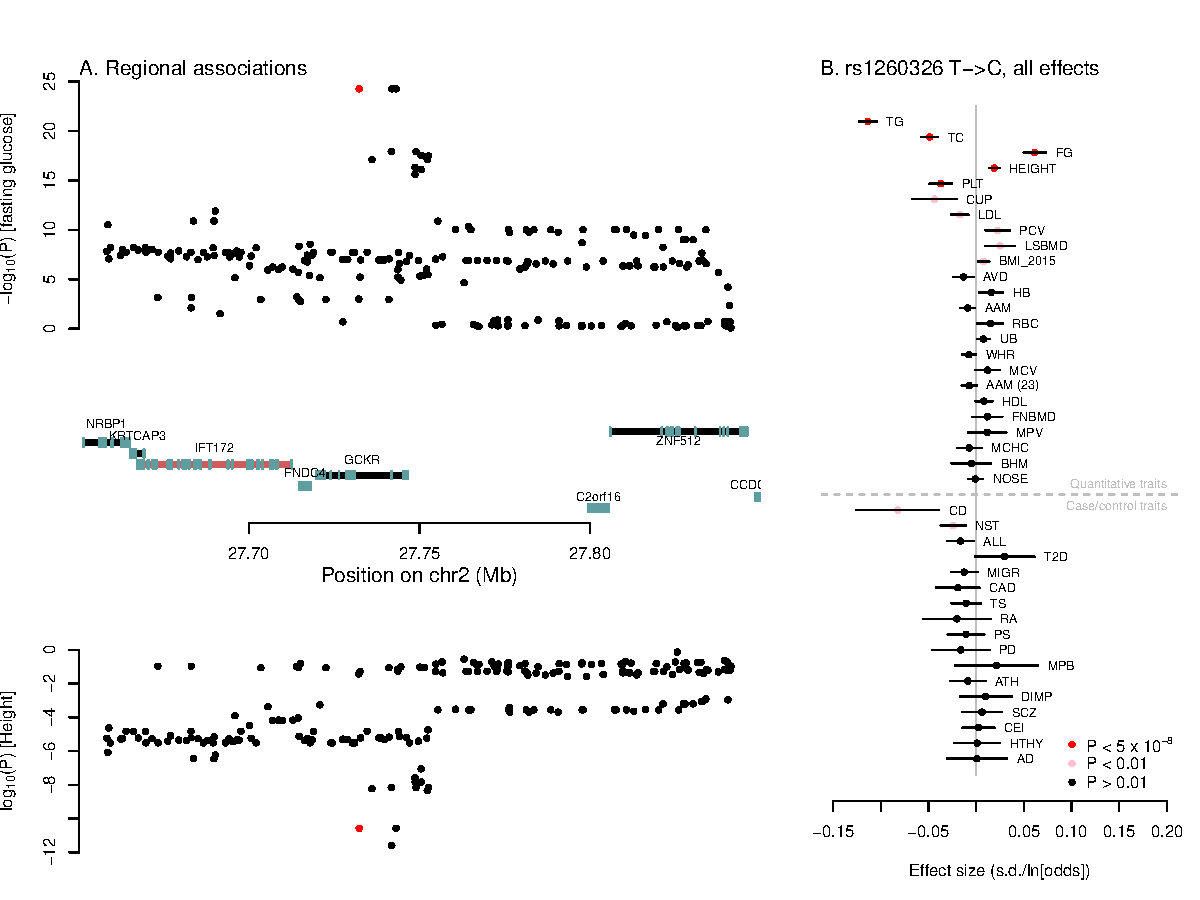
\includegraphics[scale = 0.6]{figs/GCKR_region.pdf}
\caption{. \textbf{GCKR region. A. Regional association signals.}  Shown are the P-values for association in the region for fasting glucose levels and height. In red is the nonsynonymous SNP rs1260326. \textbf{B. Effect of rrs1260326 on all phenotypes.} Shown are the effects of the C allele on all phenotypes where this variant was successfully genotypes or imputed. Bars represent 95\% confidence intervals. }\label{f_gckr}
\end{center}
\end{figure}


\begin{figure}
\begin{center}
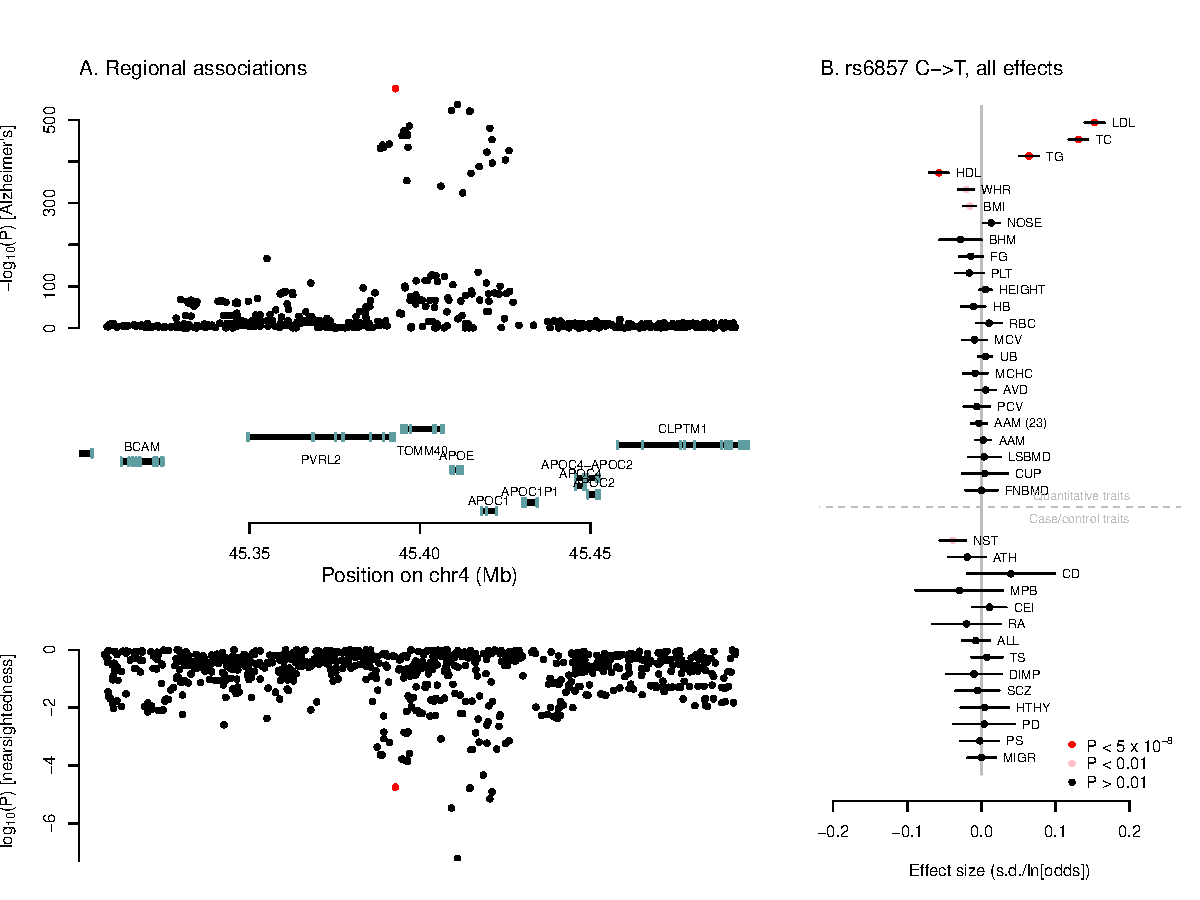
\includegraphics[scale = 0.6]{figs/APOE_region.pdf}
\caption{. \textbf{APOE region. A. Regional association signals.} Shown are the P-values for association in the region for Alzheimer's disease and nearsightedness. In red is the SNP rs6857, which tags the APOE4 allele. \textbf{B. Effect of rs6857 on all phenotypes.} Shown are the effects of the T allele on all phenotypes where this variant was successfully genotypes or imputed. Bars represent 95\% confidence intervals. For ease of display we do not show is the effect size on Alzheimer's disease, which is 1.2 (on a log-odds scale)}\label{f_apoe}
\end{center}
\end{figure}


\section{Expanded analysis of putative causally-related traits}
As noted in the main text, in our initial scan for putative causally-related traits, we identified five pairs of traits. One of these was a putative causal relationship between risk of coronary artery disease and risk of rheumatoid arthritis (Supplementary Figure \ref{f_cad_ra}). In the data used, variants that increase risk of CAD tend to decrease risk of RA (Supplementary Figure \ref{f_cad_ra}A), while variants that influence RA appear to have no correlated effects on CAD (Supplementary Figure \ref{f_cad_ra}B). This echoes the patterns seem for the other phenotypes in Figure 5 in the main text. 

However, three issues caused us to worry this correlation might be spurious. First, the number of variants identified in the GWAS of CAD was small--eleven, compared to 30 for BMI, 30 for hypothyroidism, and 41 for LDL cholesterol. Second, there appears to be no overall genome-wide genetic correlation between risk of CAD and risk of RA \citep{bulik2015atlas}. Third, this observed correlation is in the opposite direction to the known epidemiological correlation where individuals with rheumatoid arthritis are at higher risk of coronary artery disease (e.g. \citet{Maradit-Kremers:2005aa}). 

We thus identified an expanded set of loci that influence CAD risk using a larger GWAS performed using a targeted genotyping array \citep{CARDIoGRAMplusC4D-Consortium:2013aa}. We downloaded the 79,129 summary statistics from the CARDIoGRAMplusC4D Metabochip study \citep{CARDIoGRAMplusC4D-Consortium:2013aa} from \url{http://www.cardiogramplusc4d.org/downloads/}, and ran fgwas as on the original GWAS (in this case without performing any imputation). This analysis identified 70 loci associated to CAD risk at a false discovery rate of 10\%. We then compared the effect sizes of these variants on CAD risk with their effect sizes on RA risk (Supplementary Figure \ref{f_cad_ra}C). The negative correlation from Supplementary Figure \ref{f_cad_ra}A ($\rho = -0.91, P = 5.6 \times 10^{-5}$) is no longer apparent in Supplementary Figure \ref{f_cad_ra}C ($\rho = -0.21, P = 0.07$). We conclude that this apparent causal relationship between risk of CAD and risk of RA was likely a false positive driven by small numbers of variants associated with CAD. 

We next wished to test the robustness of the other inferred causal relationships. To do this, we used the fact that we discarded variants typed on the Metabochip from \citet{Locke:2015aa} for our main analysis. This was done to allow for imputation at the level of summary statistics, but resulted in a significant loss of power to identify variants since many individuals were typed using only this genotyping array. We thus re-processed the data from \citet{Locke:2015aa} as described in the main text, except that we 1) did not perform imputation, but 2) included variants typed on the Metabochip. This increased the number of loci identified at a false discovery rate of 10\% from 30 to 75. We plotted the effects of these variants on BMI and triglyceride levels (Supplementary Figure \ref{f_bmi_expanded}A), and on BMI and type 2 diabetes (Supplementary Figure \ref{f_bmi_expanded}A). The evidence for a correlation in the effect sizes of the set of 30 variants on BMI and triglyceride levels ($\rho =  0.74, P = 5.9 \times 10^{-6}$) remained strong in the set of 75 loci ($\rho = 0.59, P = 7.1 \times 10^{-8}$). Likewise, the evidence for a correlation in the effect sizes of the set of 30 variants on BMI and risk of type 2 diabetes ($\rho = 0.78, P = 1.6 \times 10^{-6}$) remained strong in the set of 75 loci ($\rho = 0.64, P = 6.2 \times 10^{-9}$). 

Interestingly, in both cases a single locus appeared as an outlier--in the case of BMI and triglycerides, a variant near APOE was associated with decreased BMI but increased levels of triglycerides (Supplementary Figure \ref{f_bmi_expanded}A), while in the case of BMI and type 2 diabetes, a variant near TCF7L2 was associated with decreased BMI but highly increased risk of type 2 diabetes (Supplementary Figure \ref{f_bmi_expanded}A, see also \citet{Helgason:2007aa}). This suggests that both the APOE locus and the TCF7L2 locus may harbor variants that influence the downstream phenotypes (triglycerides and type 2 diabetes risk, respectively) through mechanisms that are independent of BMI. More generally, variants near TCF7L2 have been used in a number of Mendelian randomization studies of type 2 diabetes (e.g. \cite{Song:2012aa, Villareal:2010aa, Pfister:2011aa}); if this locus affects multiple phenotypes via different molecular mechanisms then it may not be an appropriate ``instrument" for this type of analysis. 


\begin{figure}
\begin{center}
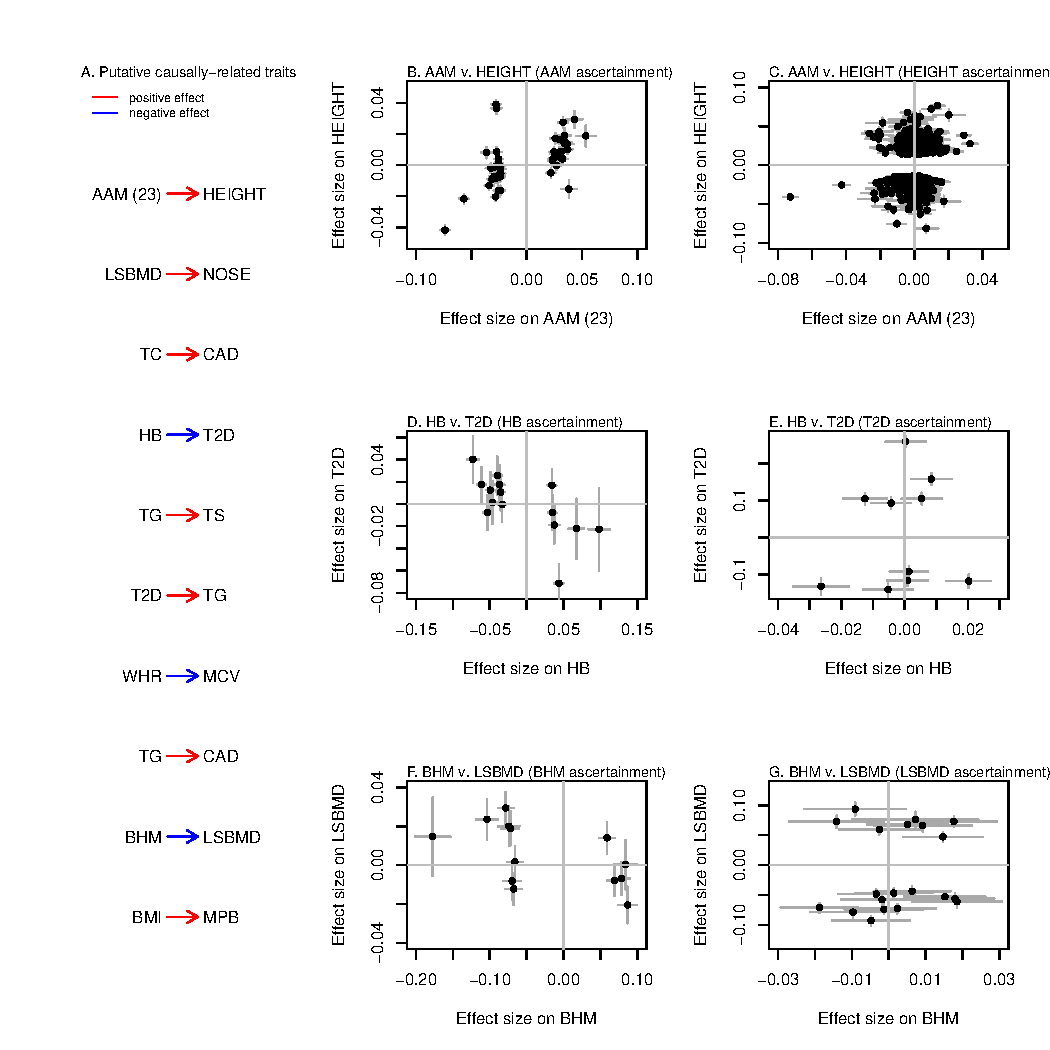
\includegraphics[scale = 0.8]{figs/causal_supp.pdf}
\caption{. \textbf{Additional pairs of traits with some evidence of a causal relationship A. List of all pairs of phenotypes.} Shown is the list of pairs of phenotypes with a relative likelihood greater than 20 (but less than 100) in favor of a causal model, ordered with the largest relative likelihood at the top. Examples of SNP effect sizes for select pairs (as in Figure 5 in the main text) are shown for age at menarche and height (\textbf{B.} and \textbf{C.}), hemoglobin levels and type 2 diabetes (\textbf{D.} and \textbf{E.}), and Beighton hypermobility and lumbar spine bone density (\textbf{F.} and \textbf{G.}) }\label{f_causal_supp}
\end{center}
\end{figure}

\begin{figure}
\begin{center}
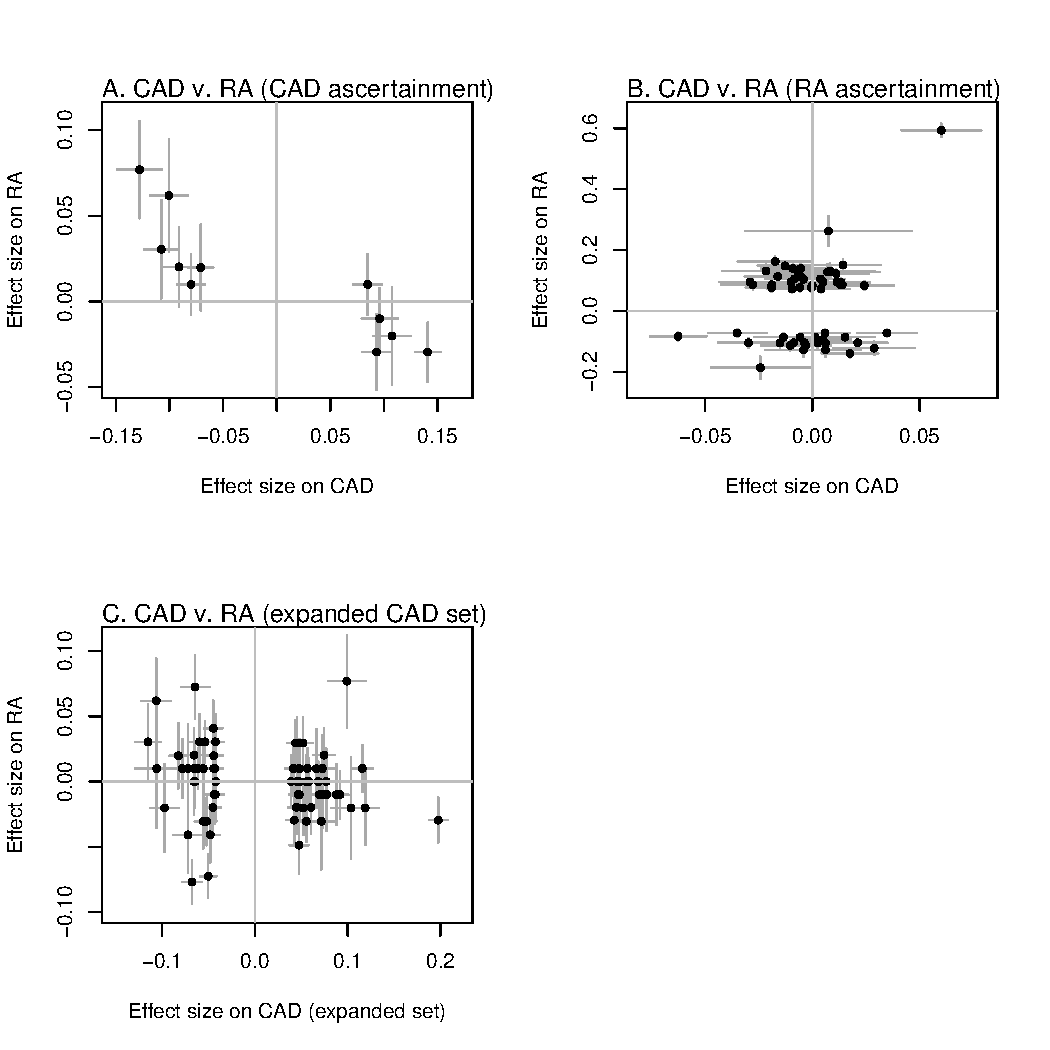
\includegraphics[scale = 0.6]{figs/cad_ra.pdf}
\caption{. \textbf{Effect sizes of genetic variants on CAD and RA.} Lines represent one standard error. \textbf{A. and B. CAD and RA, initial analysis.} The effect sizes of genetic variants on CAD and RA for variants identified in the GWAS for CAD (\textbf{A.}) or RA (\textbf{B.}). \textbf{C. Effect sizes of genetic variant on CAD and RA, expanded analysis.} Shown are the effect sizes of genetic variants on CAD and RA for variants identified in a larger GWAS for CAD, see Supplementary Text for details.} \label{f_cad_ra}
\end{center}
\end{figure}

\begin{figure}
\begin{center}
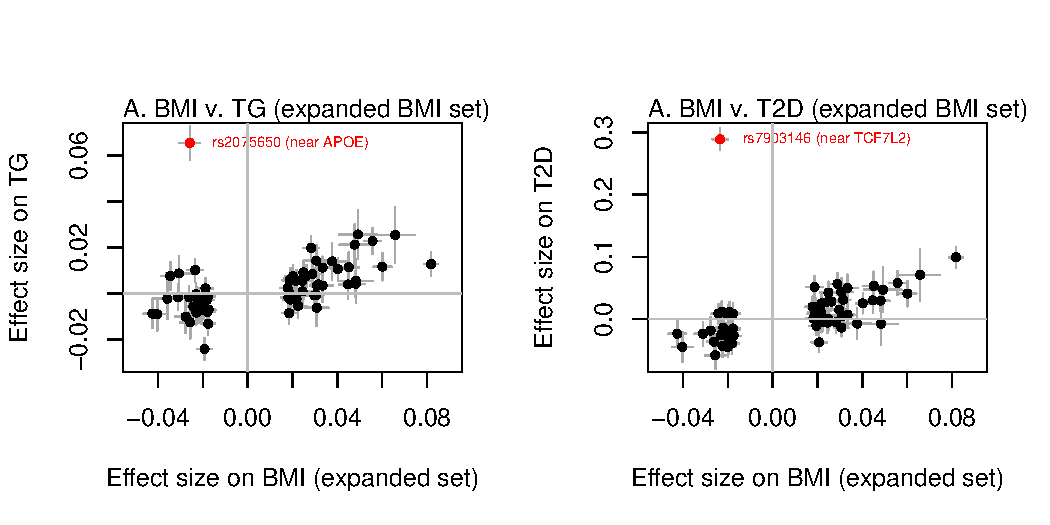
\includegraphics[scale = 0.6]{figs/bmi_expanded.pdf}
\caption{. \textbf{Effect sizes of genetic variants on BMI and A. TG or B. type 2 diabetes in a larger dataset.} Shown are the effect sizes of genetic variants on BMI and TG/T2D for variants identified in a larger GWAS for BMI, see Supplementary Text for details. In red are individual SNPs of note.}\label{f_bmi_expanded}
\end{center}
\end{figure}

\clearpage
\begin{center}
\begin{table}
\tiny{
    \begin{tabular}{| c|}
       \hline
 	See file \texttt{table\_S1.tab} \\
       \hline
        
    \end{tabular}
    }
      \caption{. \textbf{Genomic regions that contain a variant that influences more than one trait.} We identified all genomics regions that contain a variant that influences more than one trait, at a threshold of a posterior probability of association greater than 0.9. Listed are the position of each locus, the phenotypes associated with the locus, and the lead SNPs for all phenotypes.} 
\end{table}
\end{center}

\clearpage

\begin{center}
\begin{table}
\tiny{
    \begin{tabular}{| c| c| c|c| m{5cm}| m{5cm}|}
       \hline
 	chromosome & start & stop & putative causal gene & phenotypes & notes \\ \hline
     chr12 & 110336719 & 113263518 & SH2B3 & ALL, PLT, FNBMD, PCV, TS, CD, RA, HB, HTHY, LDL, HDL, RBC, TC, CAD&  often led by nonsynonymous polymorphism rs3184504, maybe two signals \\ \hline
     chr9 &135298842 & 137041122 & ABO & ALL, PCV, TS, ATH, LDL, MIGR, CEI, HB, RBC, TC, CAD &  putatively driven by an eQTL at ABO or type A1 blood, see Figure in main text\\ \hline
     chr2  & 26894985 & 28598777& GCKR &  PLT, CUP, LDL, CD, FG, TG, HEIGHT, NST, TC & often led by nonsynonymous SNP rs1260326 \\ \hline
     chr11 & 58780549 & 62223771 & none & PLT, HEIGHT, LDL, CD, FG, TG, HDL, TC & LD block covers FADS1, FADS2\\ \hline
     chr16 & 27445755  & 29036613 & none & ALL, BMI, TS, ATH, CD, RA, PD, NST & large LD block at 28-29Mb \\ \hline
     chr6  & 33236497 & 35455756 &none& CUP, BMI, LDL, MIGR, HDL, TC, CAD& LD block from 34.5-35Mb\\ \hline
     chr4  & 100678360 & 103221356 & SLC39A8 & ALL, HEIGHT, CD, PD, SCZ, HDL, NST & often led by nonsynonymous SNP rs13107325\\ \hline
     chr10 & 63341695 & 65794114 & none & PLT, BMI, HEIGHT, MPV, TG, HDL & large LD block from 65Mb-65.5Mb \\  \hline
     chr16  & 53382572 & 55903774 & none & CUP, AAM, BMI, T2D, AVD, HDL & intron of FTO \\ \hline
     chr15 & 58441366 & 59694116 & none & PCV, HB, TG, HDL, RBC, TC & nearest gene is LIPC\\ \hline
     chr19 & 44744108 & 46102697 & APOE & AD, LDL, WHR, TG, HDL, NST & covers APOE\\ \hline
     chr22  & 19912358 & 22357325 & none & HEIGHT, CD, RA, MCV, HDL, TC & covers UBE2L3, lots of gaps in SNP coverage\\ \hline
     chr6 & 89973052 & 91843196 & none & ALL, ATH, CD, DIMP, SCZ, HTHY & covers BACH2  \\ \hline
     chr4 & 87534648 & 89238028 & none & PCV, HB, TG, HDL, RBC, TC & large LD block 87.5-88Mb\\ \hline 
     chr3 & 139954597 & 141339097 & none & ALL, MPB, CD, MCV, HEIGHT, NST & LD block covers ACFL2, ZBTB38, RASA2\\ \hline
     chr1  & 7247335  & 9365199 & none & ALL, AAM, FNBMD, ATH, PD, SCZ & LD block covers RERE, SLC45A1 \\ \hline
      \hline
        
    \end{tabular}
    }
      \caption{. \textbf{Genomic regions with a variant that influences a large number of phenotypes in these data.} We sorted all genomic regions in Supplementary Table 1 (excluding the MHC region from 26-34Mb on chromosome 6, and merging the two GWAS of age at menarche) based on the number of phenotypes a single variant was predicted to influence. Shown are all regions with a variant that influences six or more traits. The "putative causal gene" is listed only when there is a nonsynonymous SNP or otherwise well-functionally characterized allele among the strongest associations in the region.} 
\end{table}
\end{center}



\bibliography{bib}
\end{document}